\subsection{Emulator sieci 5G}

\subsubsection{Open5GS}

Pierwszym komponentem emulatora jest otwartoźródłowe oprogramowanie Open5GS. Oficjalna strona projektu znajduje się tutaj: \url{https://open5gs.org/open5gs/}. Open5GS emuluje sieć rdzeniową (ang. \textit{core network}) czwartej oraz piątej generacji sieci standaryzowanych przez 3GPP. Architektura oprogramowania przedstawiona jest na rysunku \ref{fig:52-open5gs}.

\begin{figure}[!h]
    \centering 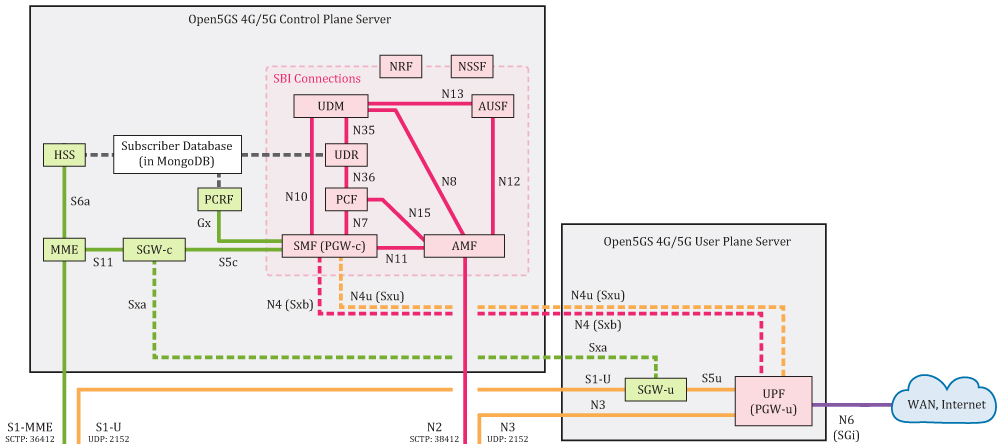
\includegraphics[width=1\linewidth]{52-open5gs.png}
    \caption{Architektura Open5GS}\label{fig:52-open5gs}
\end{figure}

\subsubsection{UERANSIM}

Drugim komponentem emulatora jest otwartoźródłowe oprogramowanie UERANSIM. Oficjalna strona projektu: \url{https://github.com/aligungr/UERANSIM}. UERANSIM symuluje Radiową Sieć Dostępową (ang. \textit{Radio Access Network (RAN)}) wraz z Terminalami Abonenta (ang. \textit{User Equipment (UE)}). UERANSIM składa się z dwóch programów \texttt{nr-ue} oraz \texttt{nr-gnb}, które mogą działać w wielu instancjach. Ich rolę w architekturze sieci 5G przedstawiono na rysunku \ref{fig:52-ueransim} w czerwonej obwódce.

\begin{figure}[!h]
    \centering 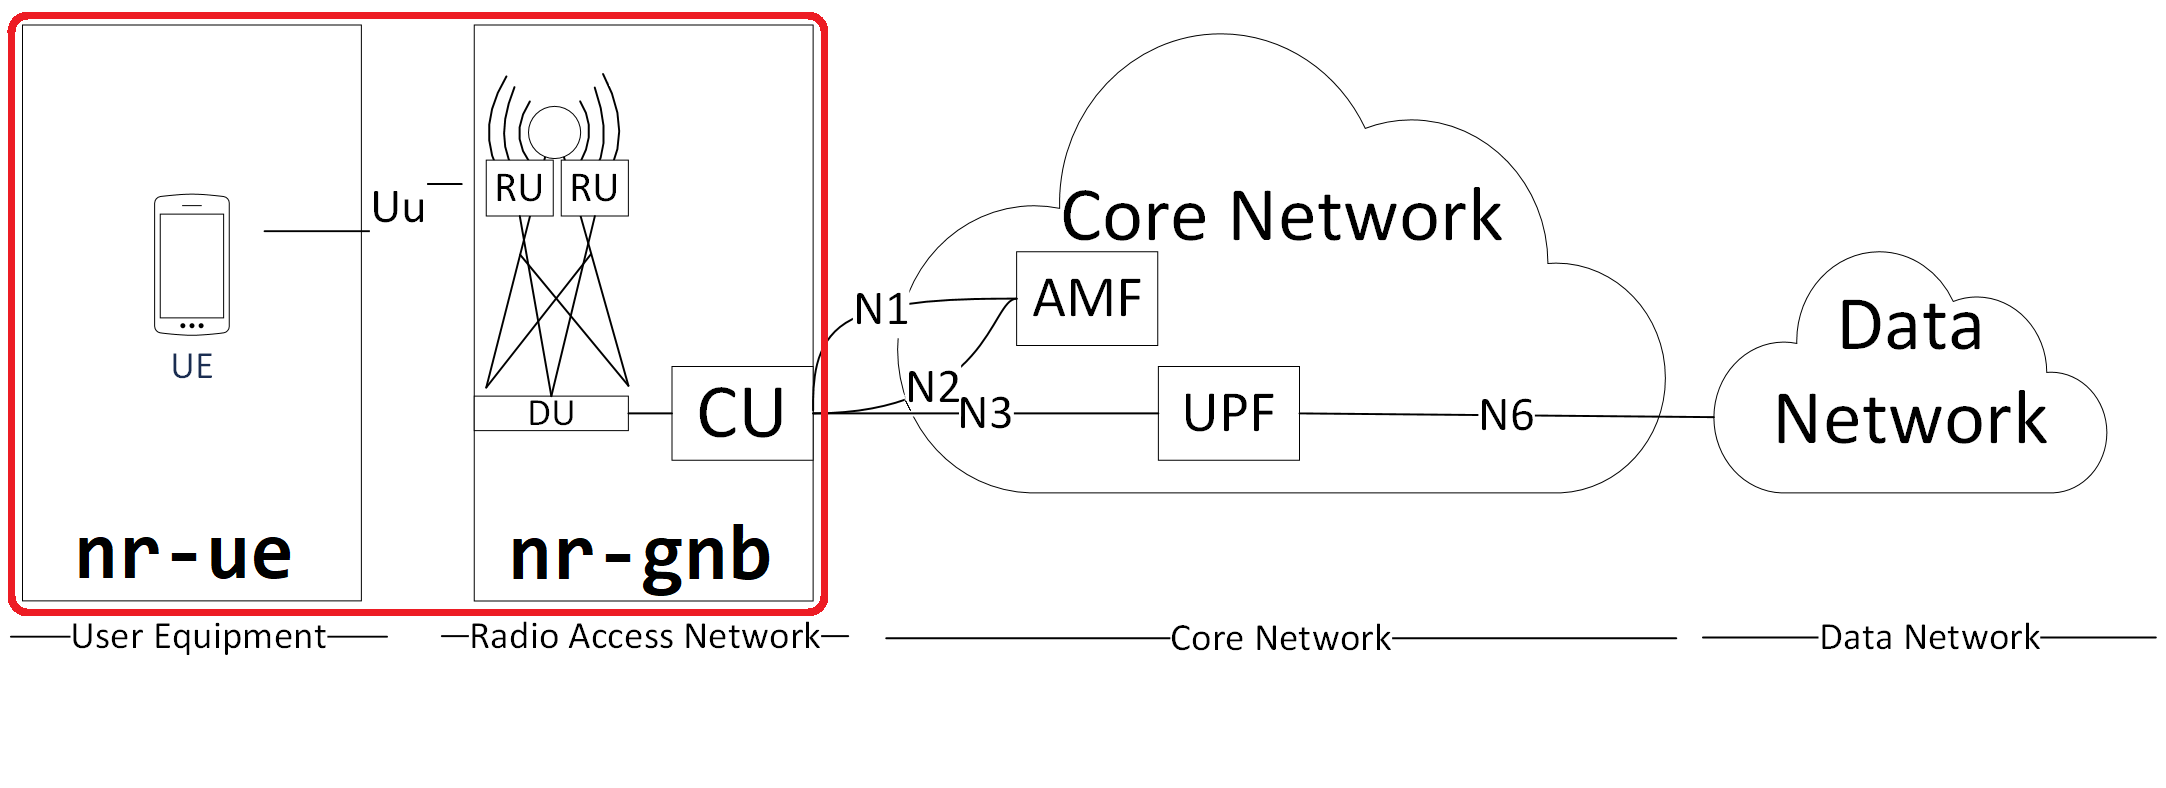
\includegraphics[width=1\linewidth]{52-ueransim.png}
    \caption{Architektura UERANSIM}\label{fig:52-ueransim}
\end{figure}

\subsubsection{Wdrożenie na Kubernetes}

Emulator sieci 5G złożony z Open5GS oraz UERANSIM wdrożono na klastrze Kubernetes według repozytorium: \url{https://github.com/niloysh/open5gs-k8s}. Przeprowadzenie kroków wskazanych w repozytorium skutkuje stanem podów w klastrze przedstawionym na rysunku \ref{fig:52-pody}.

\begin{figure}[!h]
    \centering 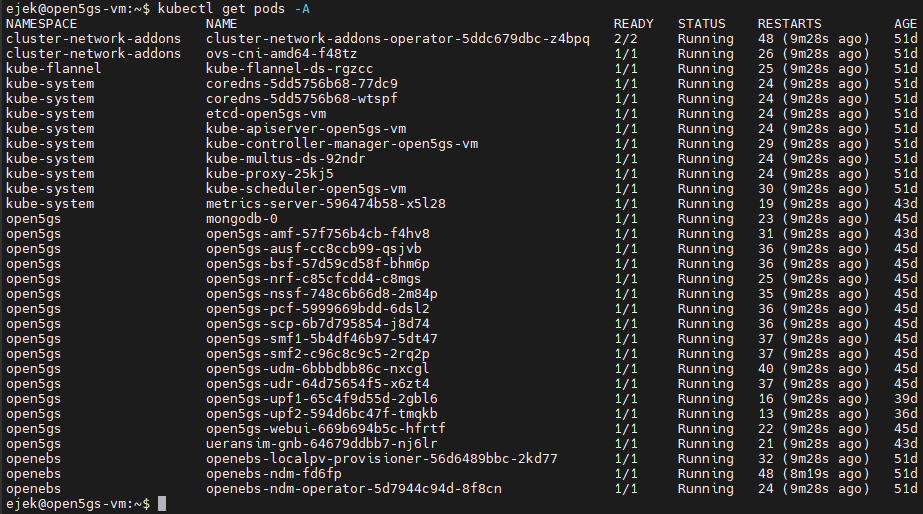
\includegraphics[width=1\linewidth]{52-pody.png}
    \caption{Stan podów w klastrze}\label{fig:52-pody}
\end{figure}

Programy UERANSIM typu \texttt{nr-ue} będą uruchamiane poza klastrem. Tej decyzji dokonano z prostego powodu. System operacyjny hostujący klaster (Ubuntu 22.04 LTS) posiada dużo większe możliwości, jeśli chodzi o narzędzia generowania ruchu, niż okrojony system operacyjny użyty w podach UERANSIM.